%!TeX root=../tese.tex
%("dica" para o editor de texto: este arquivo é parte de um documento maior)
% para saber mais: https://tex.stackexchange.com/q/78101/183146

% Vamos definir alguns comandos auxiliares para facilitar.

% "textbackslash" é muito comprido.
% \newcommand{\sla}{\textbackslash}

% Vamos escrever comandos (como "make" ou "itemize") com formatação especial.
% \newcommand{\cmd}[1]{\textsf{#1}}

% Idem para packages; aqui estamos usando a mesma formatação de \cmd,
% mas poderíamos escolher outra.
% \newcommand{\pkg}[1]{\textsf{#1}}

% A maioria dos comandos LaTeX começa com "\"; vamos criar um
% comando que já coloca essa barra e formata com "\cmd".
% \newcommand{\ltxcmd}[1]{\cmd{\sla{}#1}}

\chapter{Static Analysis}
\label{cap:static}

Understanding how social networks recommend content to users is central to the
debate around political polarization and radicalization. There are many ways of
exploring recommender systems without examining their code, from simulating
their behavior after careful observation \citep{yao_measuring_2021} to directly
collecting recommendation data \citep{ribeiro_auditing_2020}, but most of them
allow us to examine only one perspective of the algorithm at a time. This means
that studying a social network's recommendation technique has inherent
limitations.

Most of the algorithms currently employed by social media companies are trade
secrets. They are also subject to constant experimentation and tuning
\citep{noauthor_congratulations_2020}, which might render worthless any research
performed before an update to the algorithm, no matter how careful the design of
the study was.

With our experiments we aim to make a tangible contribution to the field of
recommender systems, specifically how their design might (or might not) foster
confinement dynamics and create degenerate feedback loops. If it does, this
could mean that even a relatively small fraction of the content can tip the
algorithm in its favor, amplifying their message, creating filter bubbles, and
possibly sending users on a radicalization spiral if that topic is related to
politics or other contentious subjects.

In this chapter we will analyze a recommendation system statically, that is,
without taking into account its evolution after multiple rounds of training and
learning from new data. This step is essential insofar as it generates valuable
information to better orient our dynamic analyses.

\section{Datasets}
\label{sec:datasets03}

Before discussing any experiment, it is necessary to introduce the datasets used
in the models. The main dataset explored in this dissertation is MovieLens
\citep{harper_movielens_2015}, a well-known set of movie reviews that has been
featured in many recommender system tutorials and papers for the past few years.
The full dataset, with 27,000,000 ratings applied to 58,000 movies, was enriched
by \citet{banik_movies_2017} with information about the movies' credits,
metadata, keywords, and links. The first five rows of the dataset are reproduced
in Table~\ref{tab:tab03_head}.

\begin{table}[h]
  \begin{tabular}{ |r|r|r|r| }
    \hline
    user\_id & movie\_id & rating & timestamp\\
    \hline
    1 & 1193 & 5 & 978300760\\
    \hline
    1 & 661 & 3 & 978302109\\
    \hline
    1 & 914 & 3 & 978301968\\
    \hline
    1 & 3408 & 4 & 978300275\\
    \hline
    1 & 2355 & 5 & 978824291\\
    \hline
    1 & 1197 & 3 & 978302268\\
    \hline
  \end{tabular}

  \caption{First five rows of the MovieLens dataset.}
  \label{tab:tab03_head}
\end{table}

In the end, because of technical limitations, the dataset used in this chapter
was sampled until 30,689 movies were left; this was the largest dataset that
could be processed in less than one hour by the hardware we had access to.

The second dataset, used for validation purposes only, was the Book-Crossing
Dataset \citep{ziegler_book-crossing_2004}. Just like the enriched MovieLens,
this dataset contained entries for ratings (1,149,780) applied by users
(278,858) to items (271,379 books), and information about these items like
title, author, publisher, etc. Since this dataset has was fewer ratings, there
was no need to sample it before running any experiment.

\section{Models}
\label{sec:models}

The goal of the static analysis is to test the hypothesis that even a simple
recommendation algorithm can demonstrate some sort of bias towards a subset of
of items. More specifically, given an algorithm that is user agnostic, i.e.,
that cannot be influenced by users' personal preferences, would the resulting
recommender system still favor any items? Excluding user information is
important because, as demonstrated by \citet{stoica_algorithmic_2018}, users
might have their own biases and these could get transferred on to the model; the
objective here is to understand the algorithm by itself without external
influences.

We developed five different models for this purpose, which are described below.
All of them follow the same basic behavior: after the model is trained on the
relevant dataset, it is able to take an item $i$ as input and return the $n$
items most similar to it, i.e., $n$ recommendations. For example, a
recommendation algorithm applied the present version of the MovieLens dataset
would generate a list of $30,689 \times n$ items.

This mimics YouTube's sidebar, which suggests videos similar to the one
currently being watched, with the exception that our models do not take a user's
watch history into account.

\subsection{Trivial Model}
\label{subsec:trivial}

The first model we developed is the trivial model, which is a sampler that
returns $n$ movies at random when asked for a recommendation. It is the simplest
model against which we can compare all others, since it has no mechanism to
favor one item over the next.

\subsection{Vanilla Model}
\label{subsec:vanilla}

Besides the trivial model, the simplest model that excludes user information is
the content-based recommender. In the real world this is an algorithm that is
able to identify similar items based on their metadata (description, tags, etc.)
and suggest the closest items to the one being used as input. A straightforward
way of building such an algorithm is creating a vector representation of each
item and then using a similarity metric to recommend the items most similar to
the one in question. The chosen similarity metric was cosine similarity because
of its simplicity, robustness, and ubiquity \citep{sarwar_item-based_2001}.

The main non-trivial model used in this study was the one that simply generated
vector representations for the full MovieLens dataset, without any modifications
(which is why it will henceforth be referred to as the vanilla model). The
metadata for each movie was made up of its keywords, main cast, director, and
genres. The vector transformation was very simple, with each position
representing one of the words of the corpus, and each element indicating how
many times that word appeared in the metadata for that movie. When the
recommendation for a movie was requested, the algorithm measured the cosine
similarity between it and every other movie, returning the IDs belonging to the
top $n$ most similar vectors.

\subsection{Cutoff Models}
\label{subsec:cutoff}

The vanilla model is at risk of being impacted by word frequency: for example,
movies whose metadata share rare words might be recommended less frequently than
movies whose metadata are not so unique. To mitigate this, we developed a model
with a cutoff point after which words would not be included in the vector
representation of the items anymore. Because of this feature, we called this
algorithm the cutoff model.

Three cutoff points were tested and only words with an absolute frequency larger
than or equal to $k$, $k = \{2, 5, 8\}$, could be included in the vector
representations.

\subsection{Similarity Models}
\label{subsec:similarity}

The next model we tested was intended to validate our choice of distance metric
for the vanilla model. In what we called similarity models, we used other
distance metrics besides cosine similarity \citep{ricci_introduction_2011}:
cosine distance, Euclidean distance and Manhattan distance. The goal here was to
verify whether other metrics could do a better (or worse) job at not creating a
subset of movies that ended up more recommended than the rest.

\subsection{Vanilla Model with Synthetic Metadata}
\label{subsec:synthetic}

The last model we developed was actually the vanilla model trained on a
variation of the original dataset. This validation step was necessary in order
to guarantee that the intrinsic properties of our data were not having an effect
on the recommendation profiles of our previous models.

The new dataset had synthetic (i.e., randomly generated) metadata: the metadata
text for each item was comprised of random words sampled uniformly from the full
metadata corpus. In the case of the MovieLens dataset, the baseline probability
of any given word $w_i$ being added to the metadata of a movie was equal to
$\overline{P(w)}$, the average probability over every word in the original
corpus.

In addition to this baseline probability, two extra sets of metadata were
constructed: one where each word was 10 times more likely to be selected than
$\overline{P(w)}$, and another where each word was 100 times more likely. All
three constructed datasets can be concisely described through the expression
$P(w_i) = C \times \overline{P(w)}, C = \{1, 10, 100\}$.

\section{Experiments}
\label{sec:experiments}

In order to evaluate these recommendation systems, at least qualitatively, we
can compare their recommendation profiles: a summary of how many times each item
is recommended overall by the model. To create this profile, the model is asked
to return $n = 10$ recommendations for each item in the dataset according to its
internal similarity metric.

The recommendation profile of the model is the number of times each item showed
up in the full set of recommendations arranged by ranking (i.e., from most
recommended to least recommended). After this computationally intensive
calculation, the occurrence of each ID would be counted and ranked accordingly
to facilitate interpretation of results, that is, the movie ranked number 1
would be the movie featured the most times in the set of all recommendations,
and so forth for every other rank.

This operation is very costly, approaching $O(MN)$ complexity, where $M$ is the
number of users in the dataset and $N$ is the number of distinct movies.

The baseline for the visualizations presented in this section is MovieLens'
original review distribution. Figure~\ref{fig:fig03_review_profile} ranks every
movie in the original dataset by their review count, i.e., the number of users
that reviewed each movie. It is important to note that we are not taking user
ratings into account for these profiles and this is deliberate: social networks
like YouTube seem to mostly ignore explicit user feedback when making
recommendations \citep{noauthor_mozilla_nodate}.

\begin{figure}
  \centering
  \begin{subfigure}{0.45\textwidth}
    \centering
    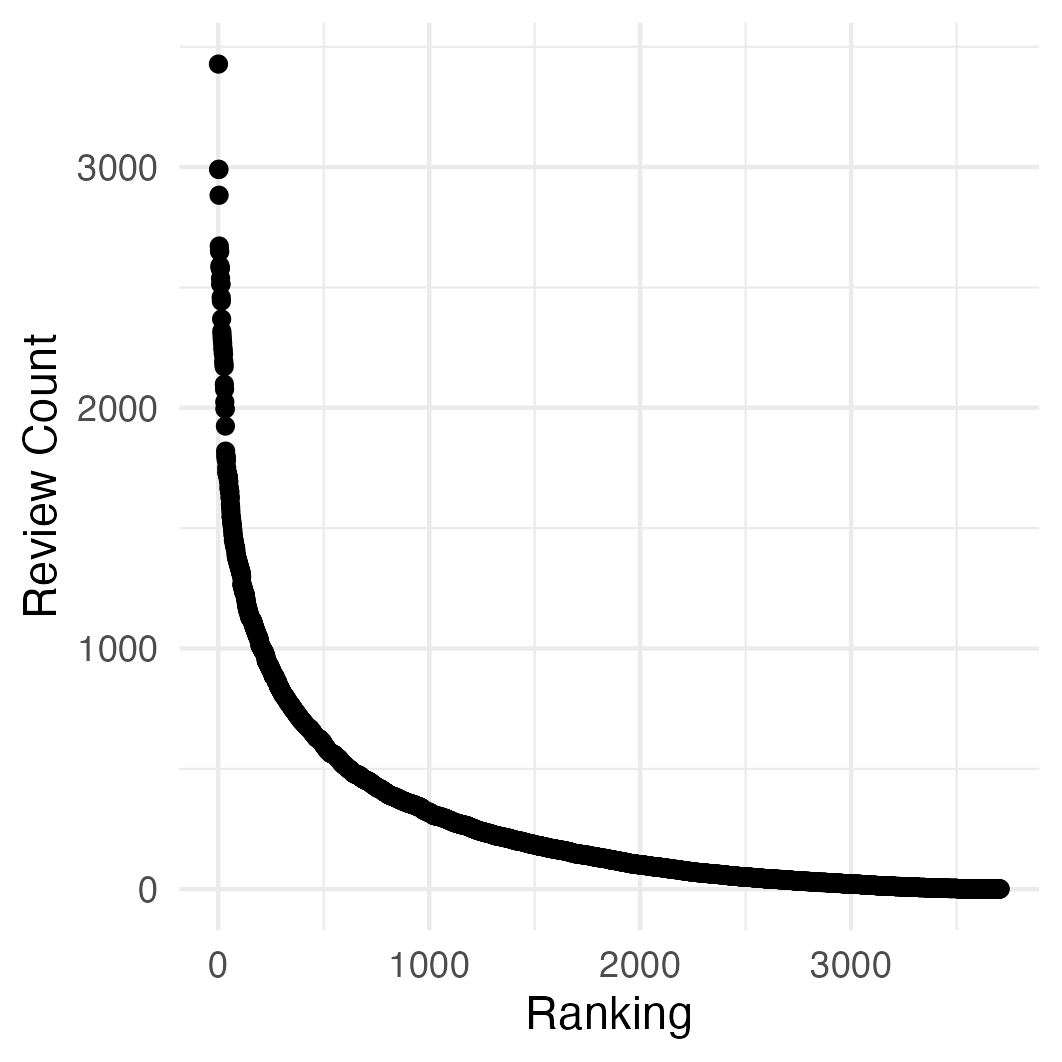
\includegraphics[width=\textwidth]{03_review_profile}
    \caption{Review profile.\label{fig:fig03_review_profile}}
  \end{subfigure}
  \begin{subfigure}{0.45\textwidth}
    \centering
    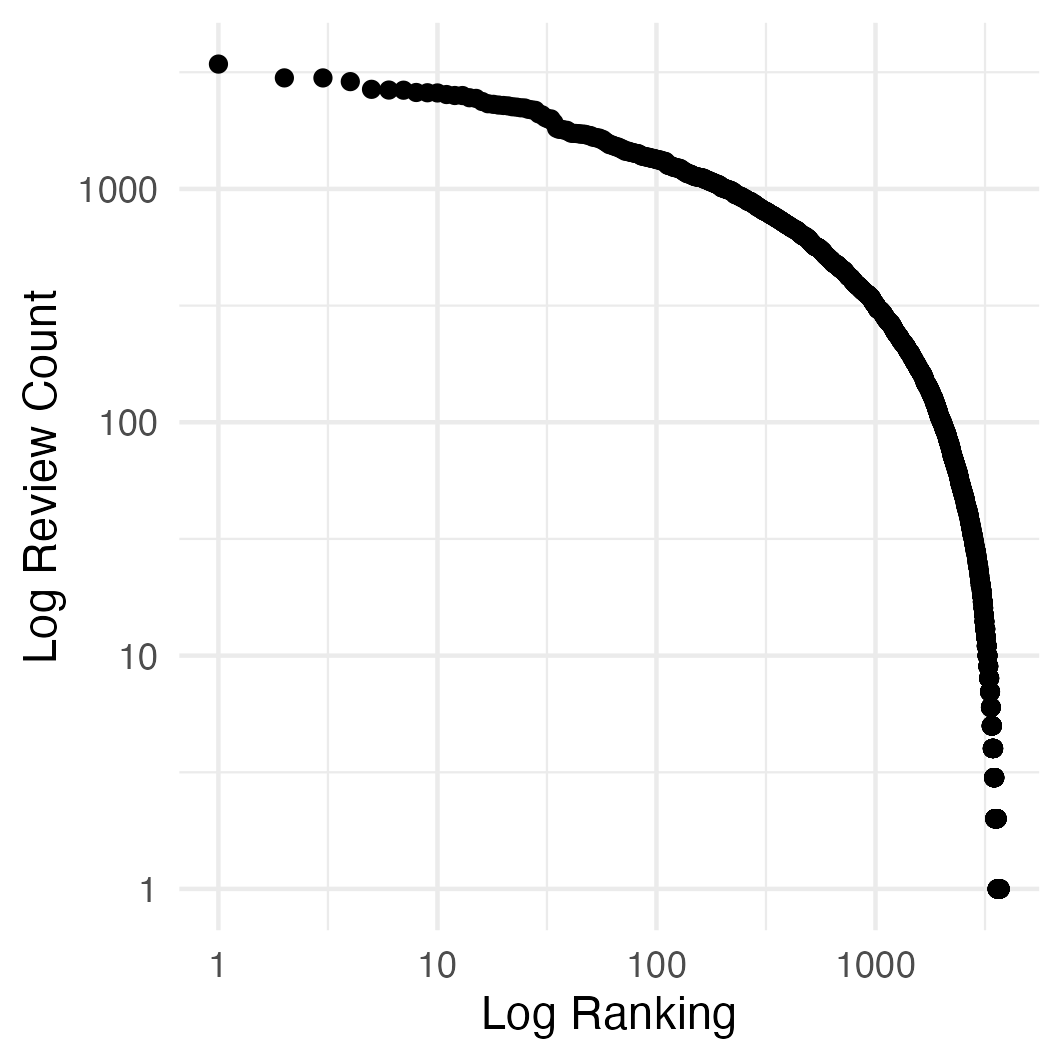
\includegraphics[width=\textwidth]{03_log_review_profile}
    \caption{Log-log plot.\label{fig:fig03_log_review_profile}}
  \end{subfigure}
  \caption{Review profile for the full dataset (a) and log-log
  plot (b).\label{fig:fig03_review_profile_both}}
\end{figure}

\subsection{Trivial Model}
\label{subsec:trivial}

Its recommendation profile can be seen in Figure~\ref{fig:fig1} and, since it is
the sum of many uniform samples, the number of times each movie is recommended
approaches a normal distribution and, therefore, the recommendation profile also
approaches the cumulative distribution function (CDF) of said distribution. The
most recommended movie appeared 25 times in the final list, while the least
recommended movie did not appear at all. Figure~\ref{fig:fig1b} shows the
log-log plot of the recommendation profile.

\begin{figure}
  \centering
  \begin{subfigure}{0.45\textwidth}
    \centering
    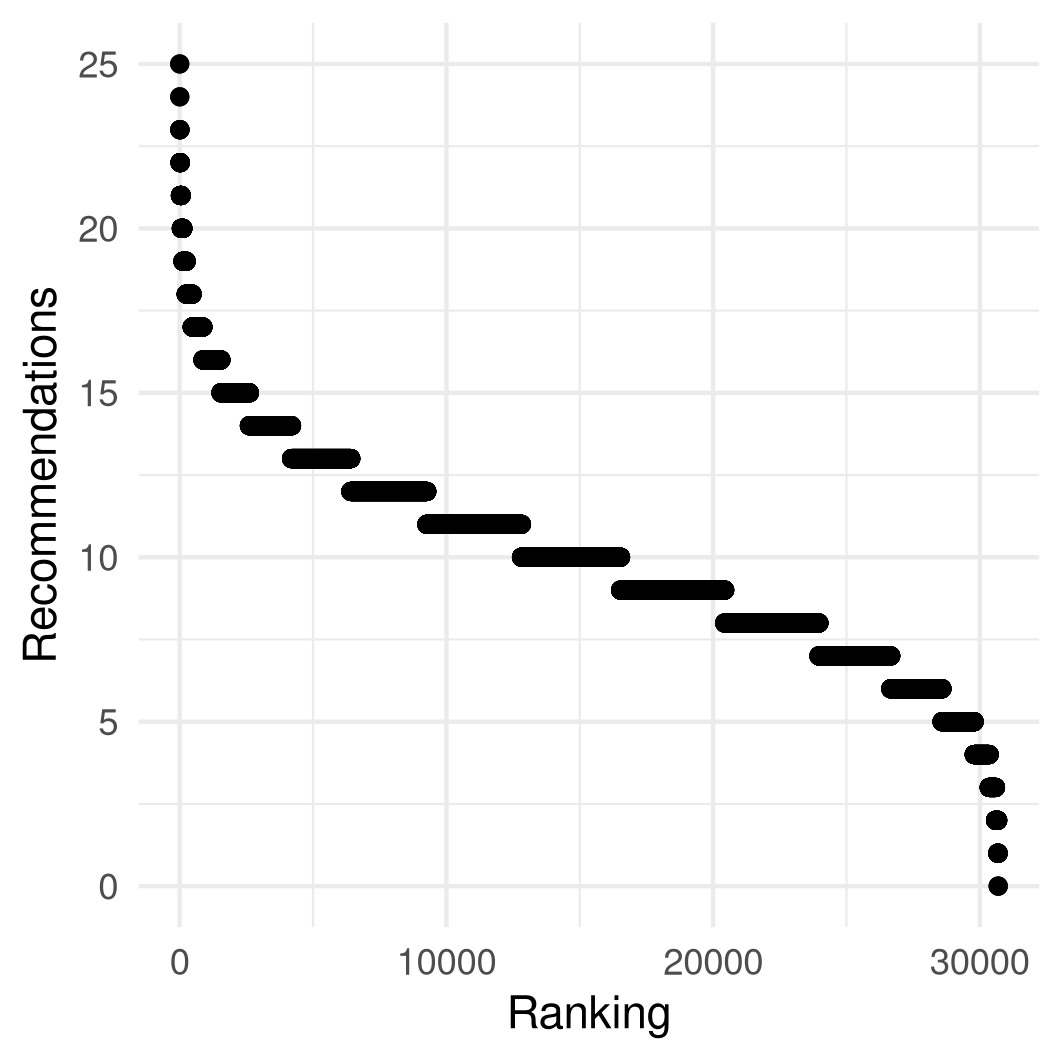
\includegraphics[width=\textwidth]{1a_random}
    \caption{Recommendation profile.\label{fig:fig1a}}
  \end{subfigure}
  \begin{subfigure}{0.45\textwidth}
    \centering
    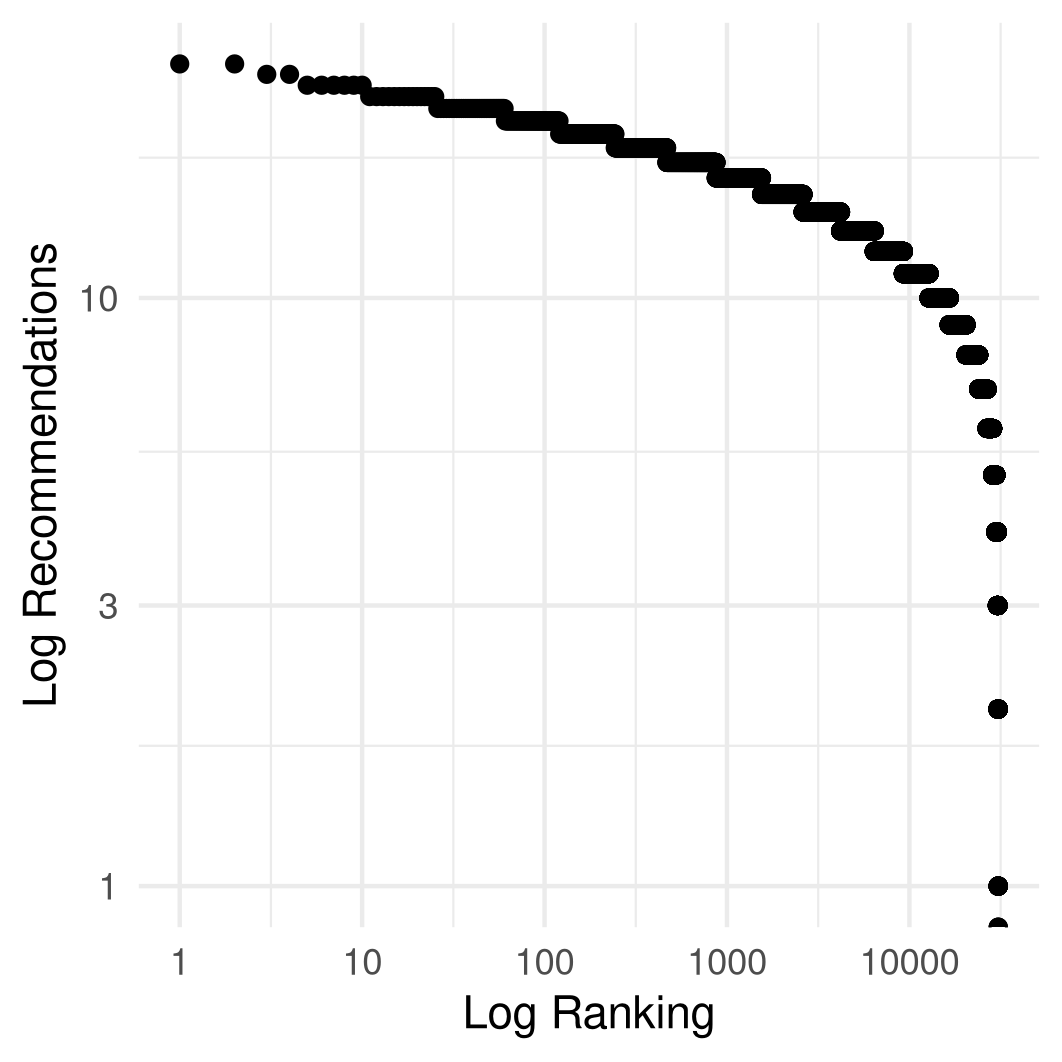
\includegraphics[width=\textwidth]{1b_random_log}
    \caption{Log-log plot.\label{fig:fig1b}}
  \end{subfigure}
  \caption{Recommendation profile for the trivial model (a) and log-log plot
    (b).\label{fig:fig1}}
\end{figure}

\subsection{Vanilla Model}
\label{subsec:vanilla}

The recommendation profile for the vanilla model can be seen in
Figure~\ref{fig:fig2a}. Here, the movie ranked number 1 appeared more than 2000
times in the full list of recommendations, with an almost exponential decrease
in the number of appearances from then on, as made evident by the log-log plot
on Figure~\ref{fig:fig2b}. This recommendation profile is a big departure from
the trivial model discussed above.

\begin{figure}
  \centering
  \begin{subfigure}{0.45\textwidth}
    \centering
    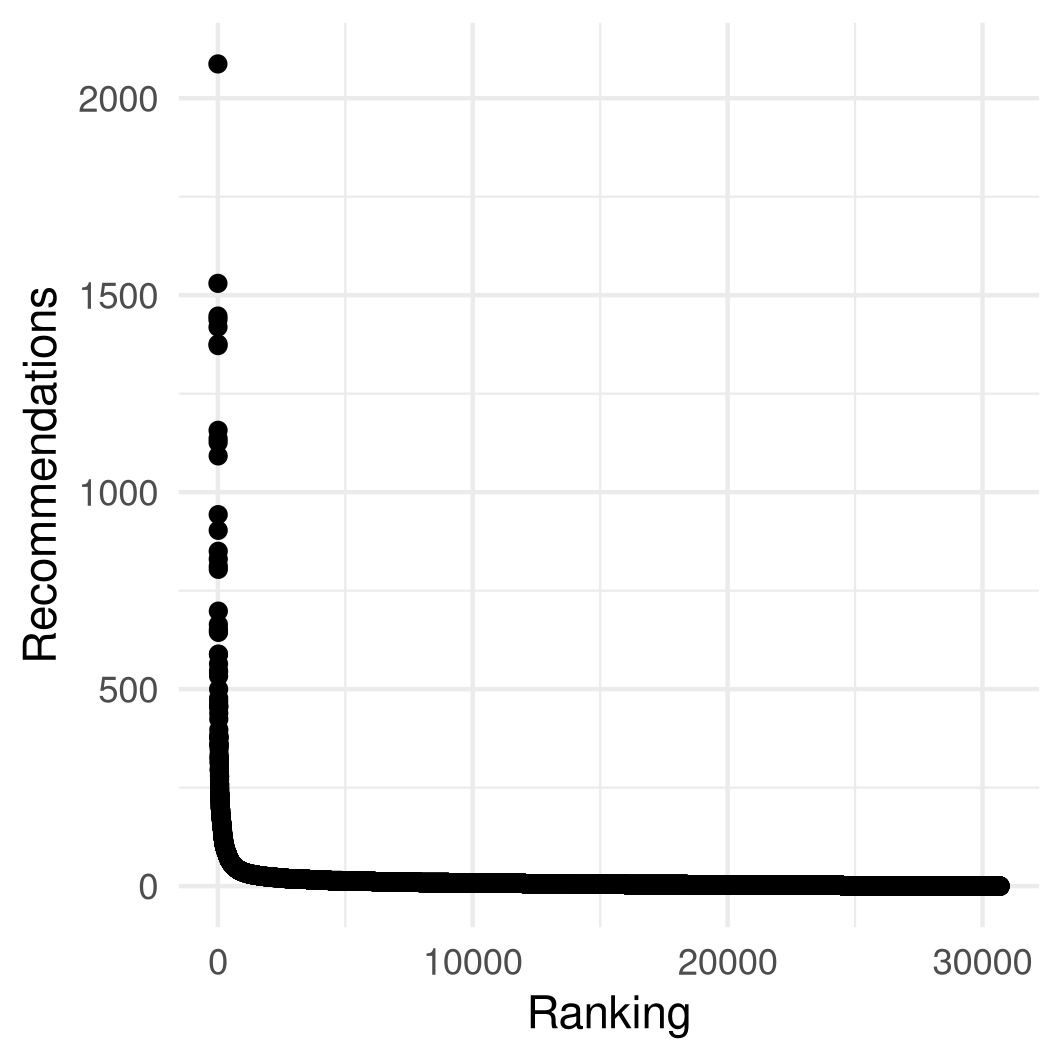
\includegraphics[width=\textwidth]{2a_vanilla}
    \caption{Recommendation profile.\label{fig:fig2a}}
  \end{subfigure}
  \begin{subfigure}{0.45\textwidth}
    \centering
    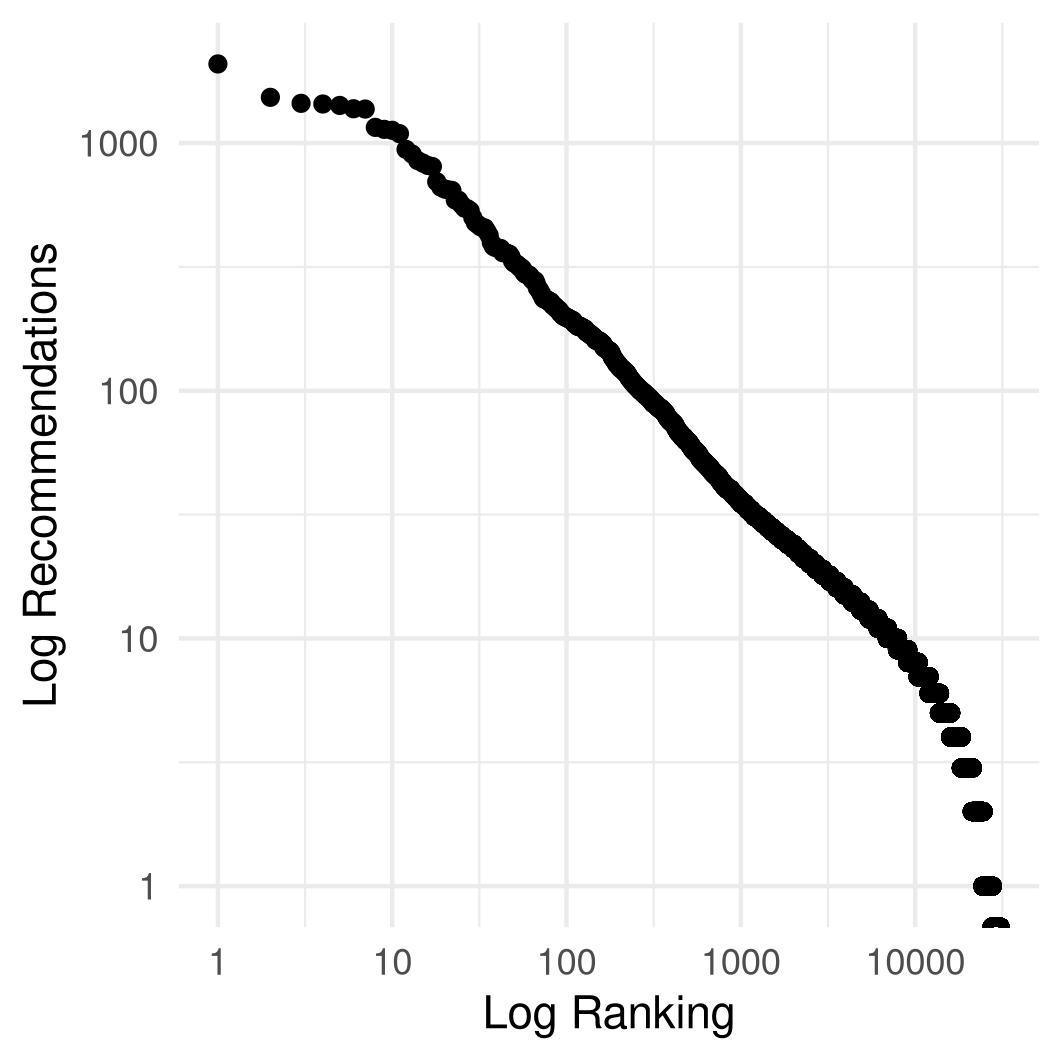
\includegraphics[width=\textwidth]{2b_vanilla_log}
    \caption{Log-log plot.\label{fig:fig2b}}
  \end{subfigure}
  \caption{Recommendation profile for the vanilla model (a) and log-log plot
    (b).\label{fig:fig2}}
\end{figure}

\subsection{Cutoff Models}
\label{subsec:cutoff}

A potential explanation for the difference between trivial and vanilla could
reside in the least used terms in the metadata and that is why we developed the
cutoff model. The results can be seen in Figure~\ref{fig:fig3} and, aside from
variations in the $y$-intercept, all plots are qualitatively very similar to
Figure~\ref{fig:fig2a}, indicating that rare words probably are not to blame for
the exponential-like decay.

\begin{figure}
  \centering
  \begin{subfigure}{0.3\textwidth}
    \centering
    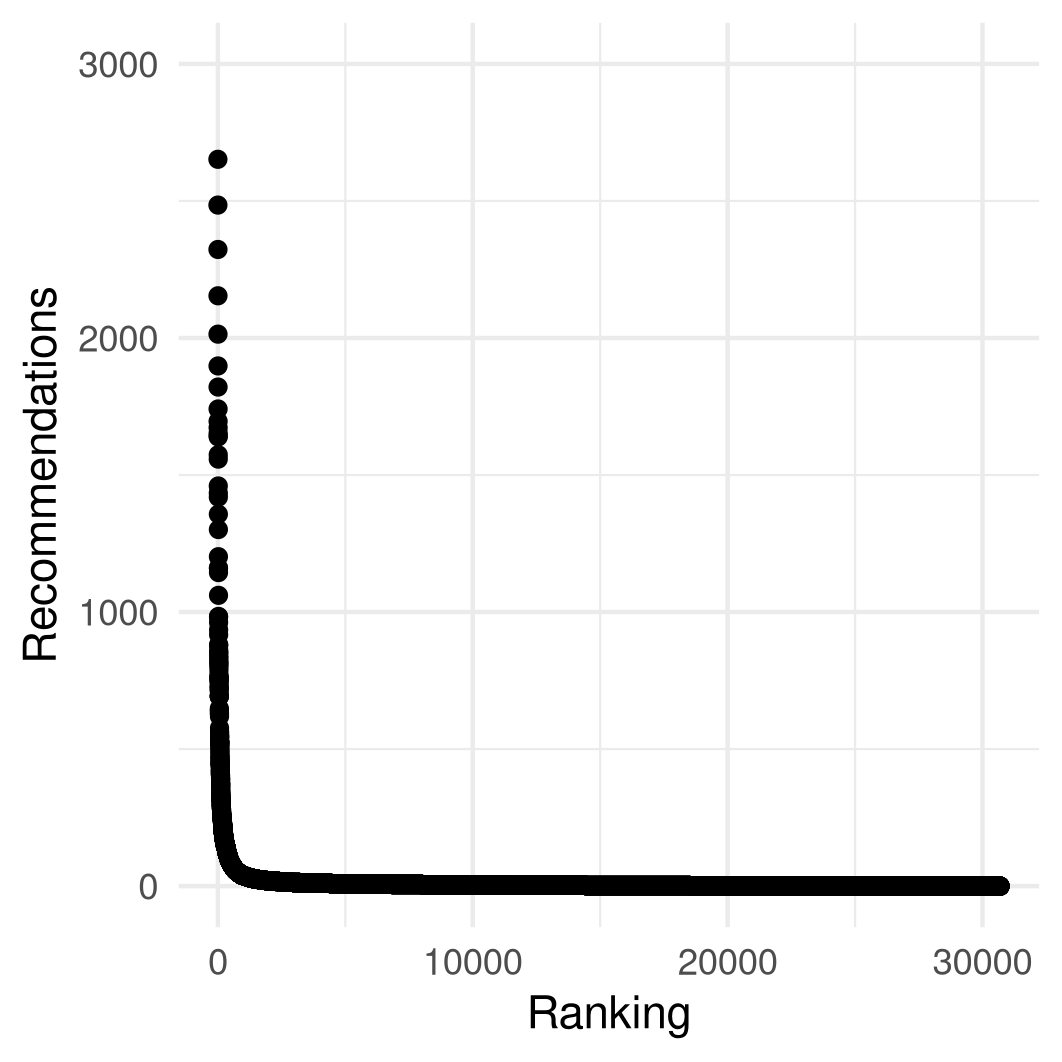
\includegraphics[width=\textwidth]{3a_cutoff_low}
    \caption{Cutoff $k = 2$.\label{fig:fig3a}}
  \end{subfigure}
  \begin{subfigure}{0.3\textwidth}
    \centering
    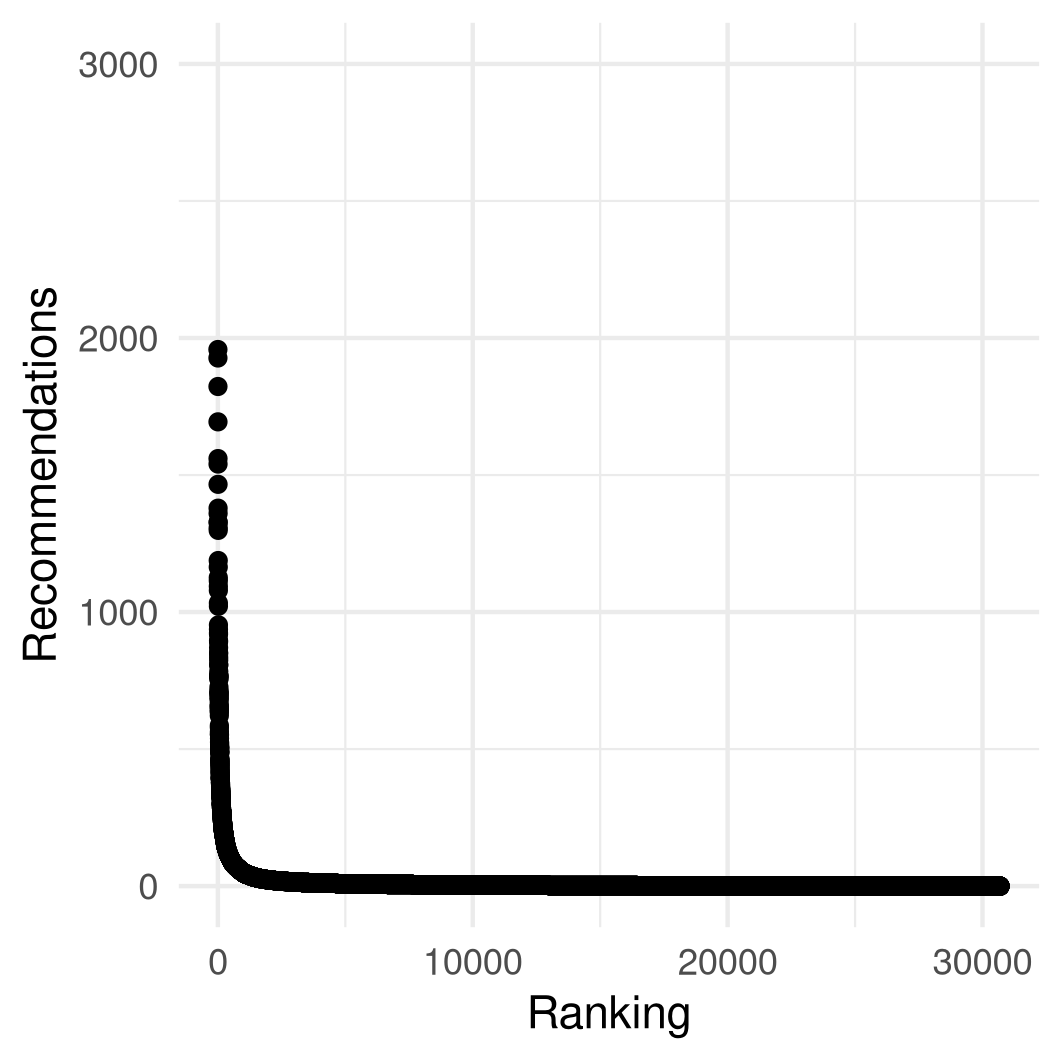
\includegraphics[width=\textwidth]{3b_cutoff_med}
    \caption{Cutoff $k = 5$.\label{fig:fig3b}}
  \end{subfigure}
  \begin{subfigure}{0.3\textwidth}
    \centering
    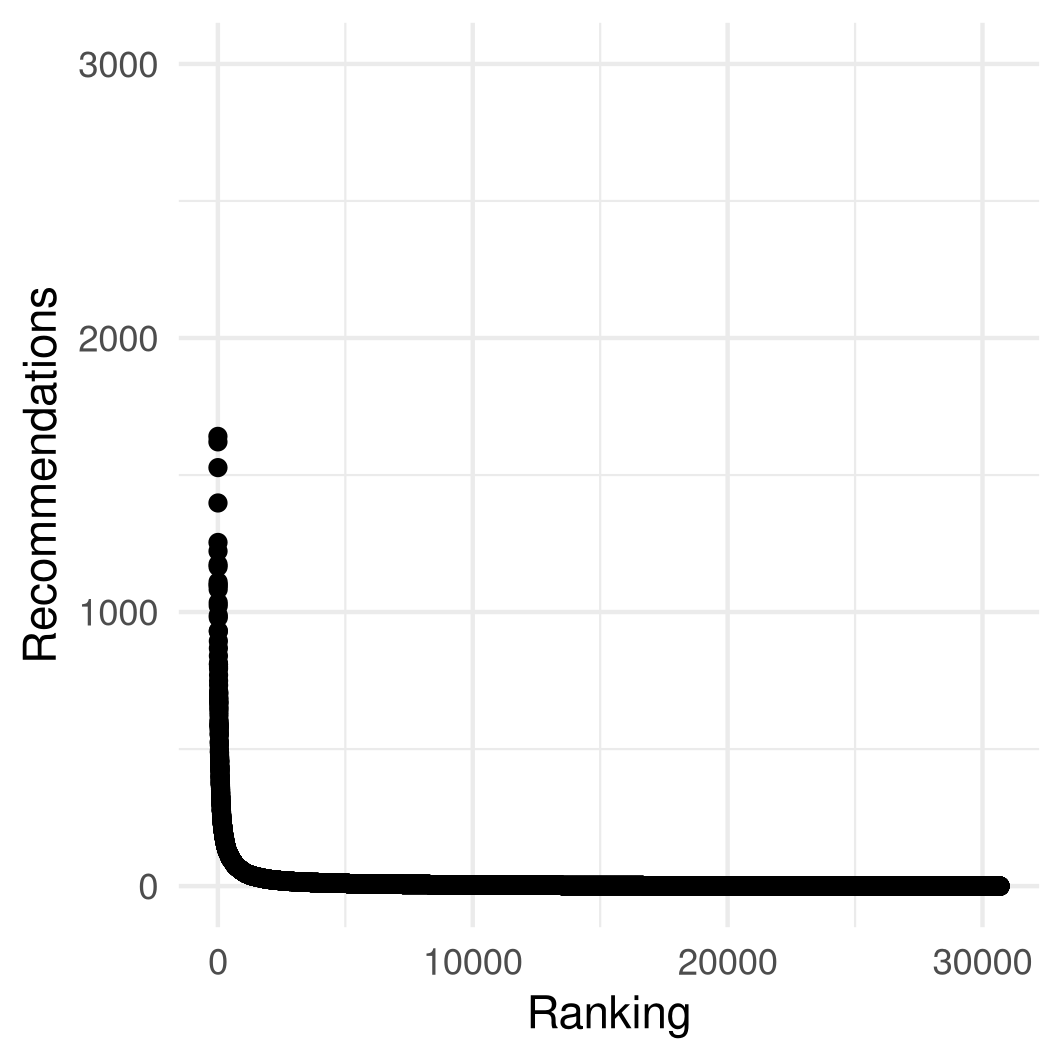
\includegraphics[width=\textwidth]{3c_cutoff_high}
    \caption{Cutoff $k = 8$.\label{fig:fig3c}}
  \end{subfigure}
  \caption{Recommendation profile for cutoff $k = 2$ (a), $5$ (b), and $8$
    (c).\label{fig:fig3}}
\end{figure}

\subsection{Similarity Models}
\label{subsec:similarity}

Since the similarity metric could also be a source of the strange behavior of
the recommendation profile, we conceived the three similarity models described
in the last section. Figure~\ref{fig:fig4} showcases a comparison between cosine
distance, euclidean distance and manhattan distance. It is clear that there are
no meaningful differences between the recommendation profiles generated by each
metric.

\begin{figure}
  \centering
  \begin{subfigure}{0.3\textwidth}
    \centering
    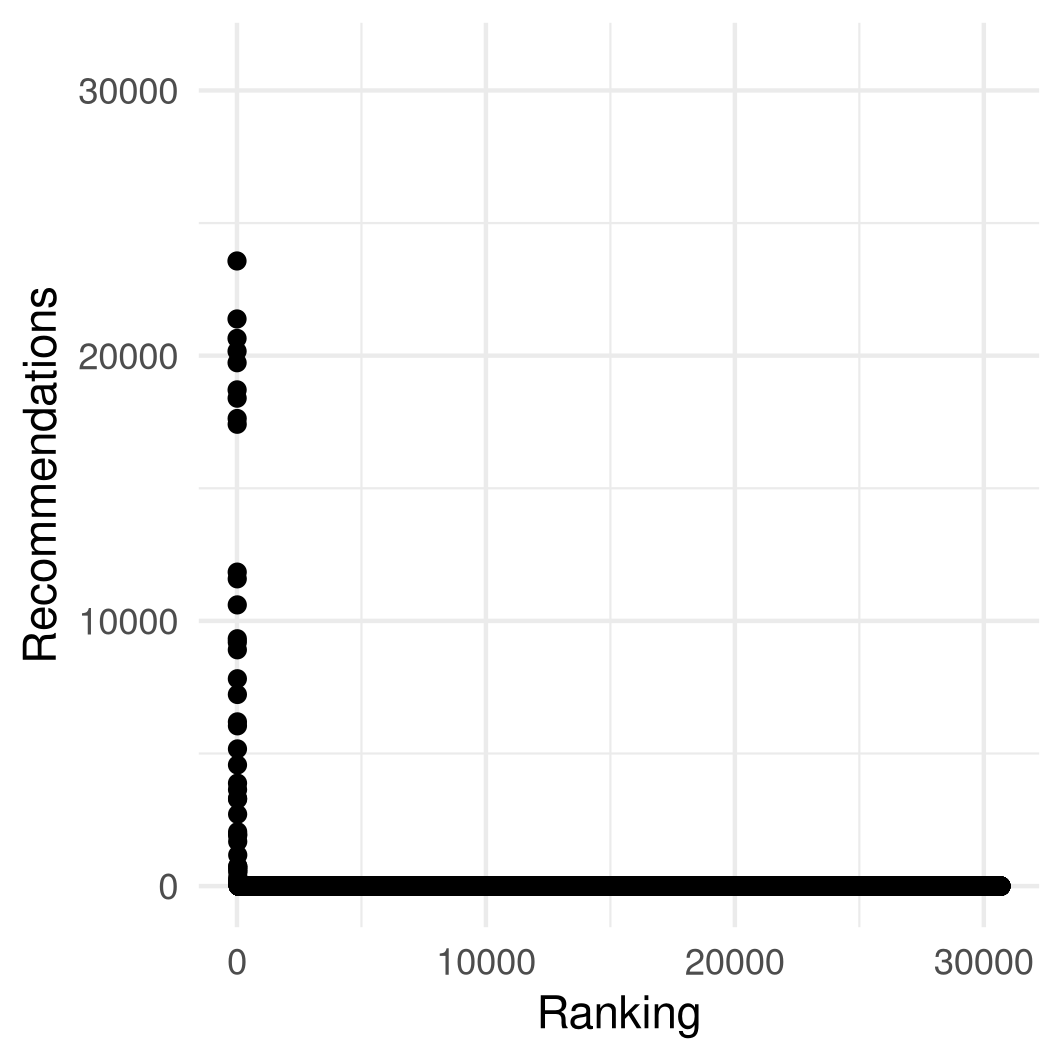
\includegraphics[width=\textwidth]{4a_cosine}
    \caption{Cosine distance (vanilla).\label{fig:fig4a}}
  \end{subfigure}
  \begin{subfigure}{0.3\textwidth}
    \centering
    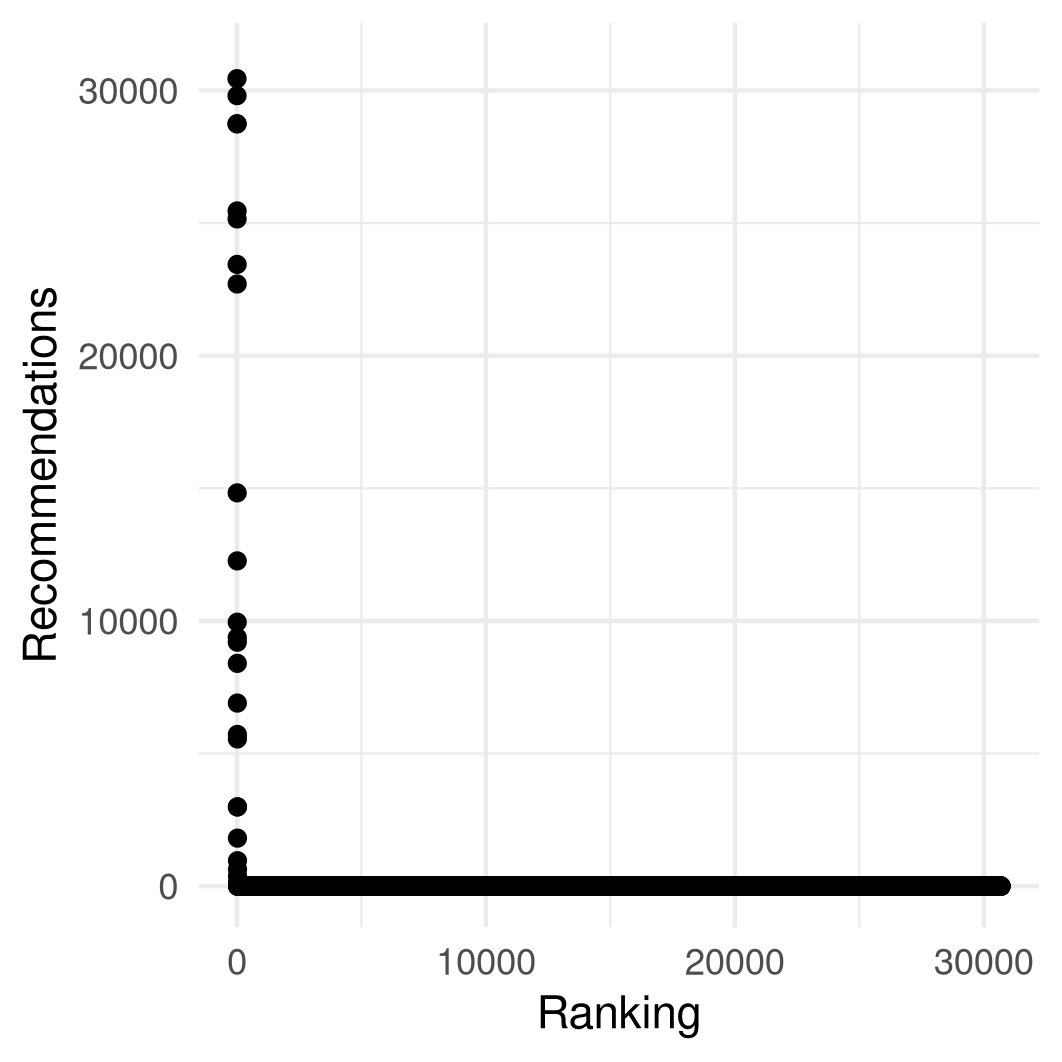
\includegraphics[width=\textwidth]{4b_euclidean}
    \caption{Euclidean distance.\label{fig:fig4b}}
  \end{subfigure}
  \begin{subfigure}{0.3\textwidth}
    \centering
    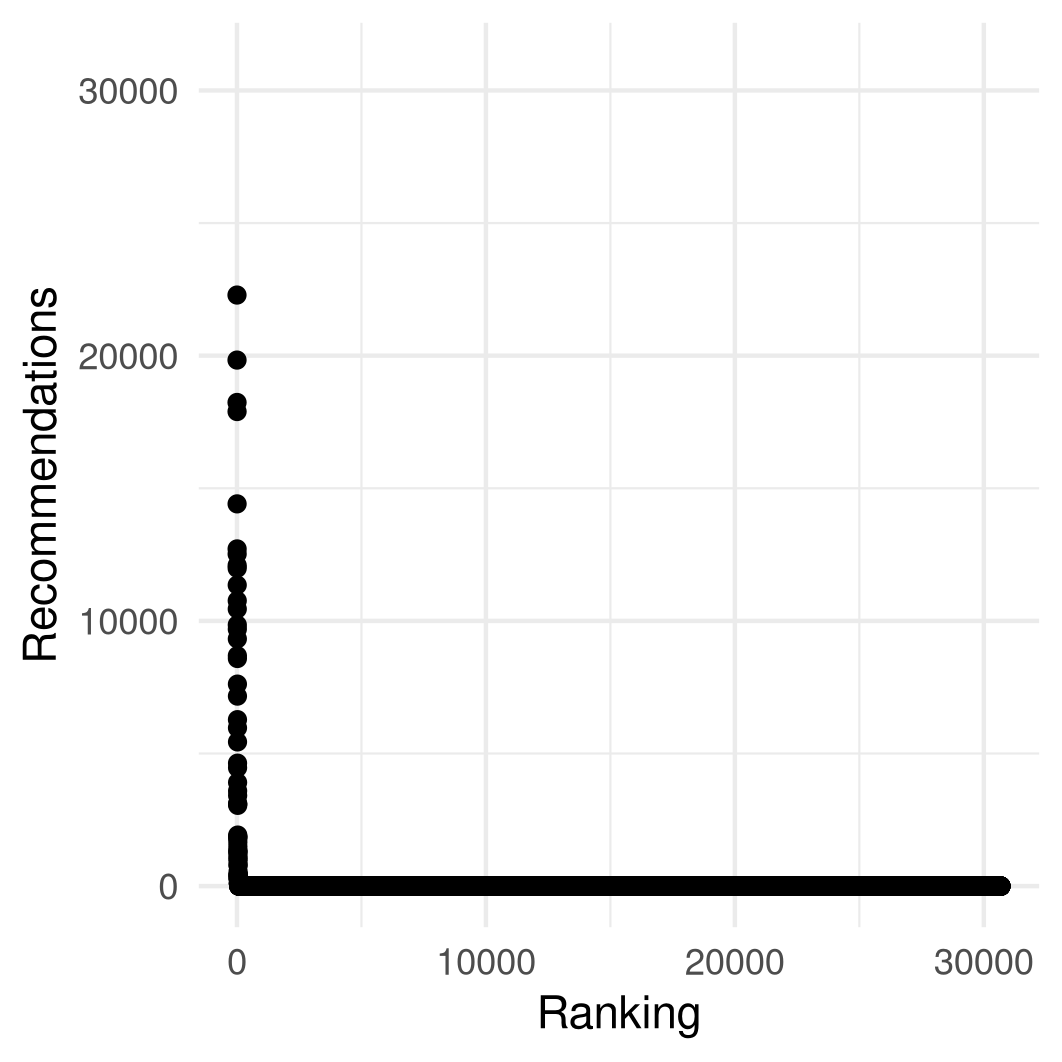
\includegraphics[width=\textwidth]{4c_manhattan}
    \caption{Manhattan distance.\label{fig:fig4c}}
  \end{subfigure}
  \caption{Recommendation profile for cosine (a), euclidean (b), and manhattan
    (c) distances.\label{fig:fig4}}
\end{figure}

\subsection{Vanilla Model with Synthetic Metadata}
\label{subsec:synthetic}

At this point it is safe to say that the type of decay seen in recommendation
frequencies up until now is not spurious and must have a clear cause. To better
investigate whether word frequency had an impact on the recommendation profiles
another hypothesis was taken into consideration: do sparser metadata cause the
recommendation curves to display a steep left-hand side?

Figure~\ref{fig:fig5} displays the recommendation profiles for the vanilla model
applied to datasets with synthetic metadata. Concretely, the figures are
equivalent to creating random metadata for the movies where the probability of
any single word being selected was approximately $1.54 \times 10^{-4}$, $1.54
\times 10^{-3}$, and $1.54 \times 10^{-2}$ respectively. The results do support
the aforementioned hypothesis since less sparse vectors indeed generated less
exponential decays.

\begin{figure}
  \centering
  \begin{subfigure}{0.3\textwidth}
    \centering
    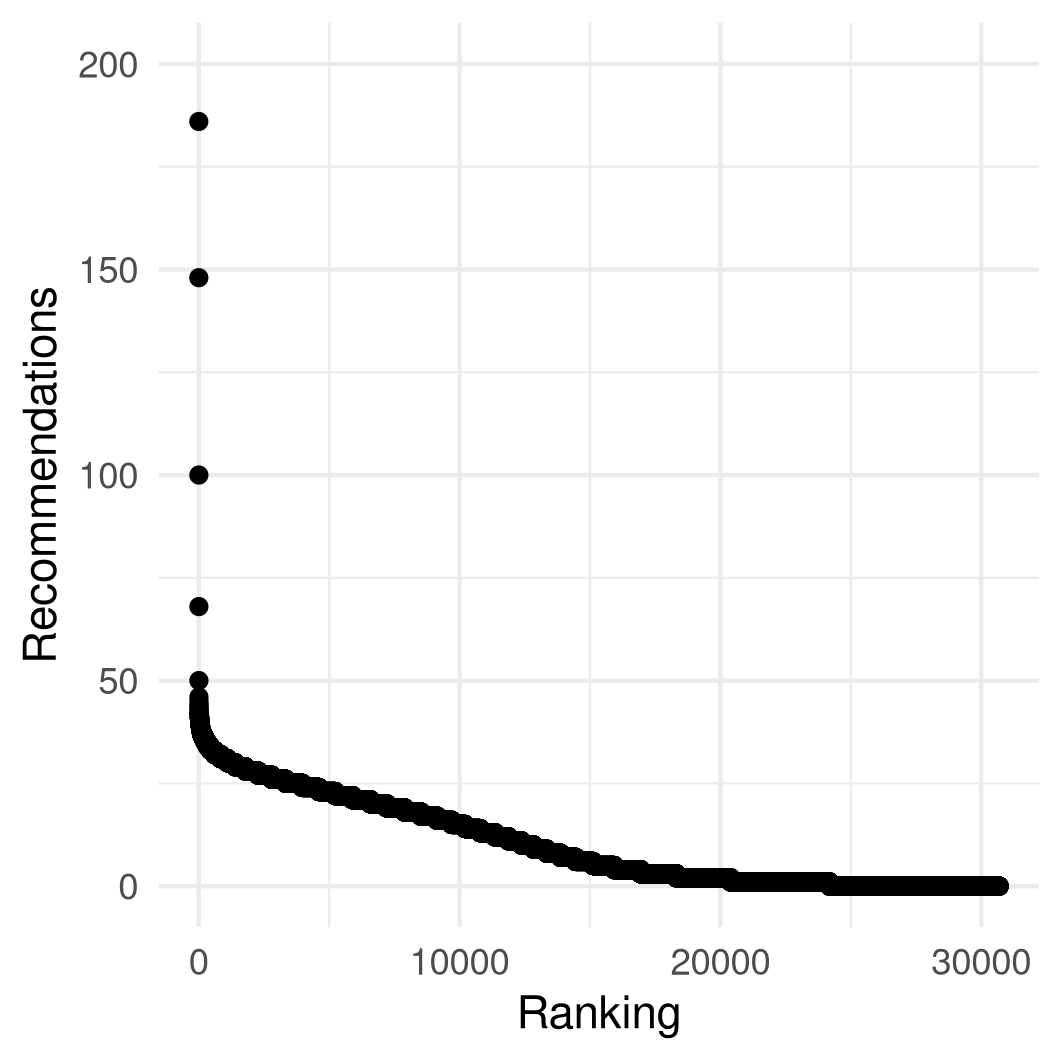
\includegraphics[width=\textwidth]{5a_p}
    \caption{$P(w_{i}) = 1 \times \overline{P(w)}$.\label{fig:fig5a}}
  \end{subfigure}
  \begin{subfigure}{0.3\textwidth}
    \centering
    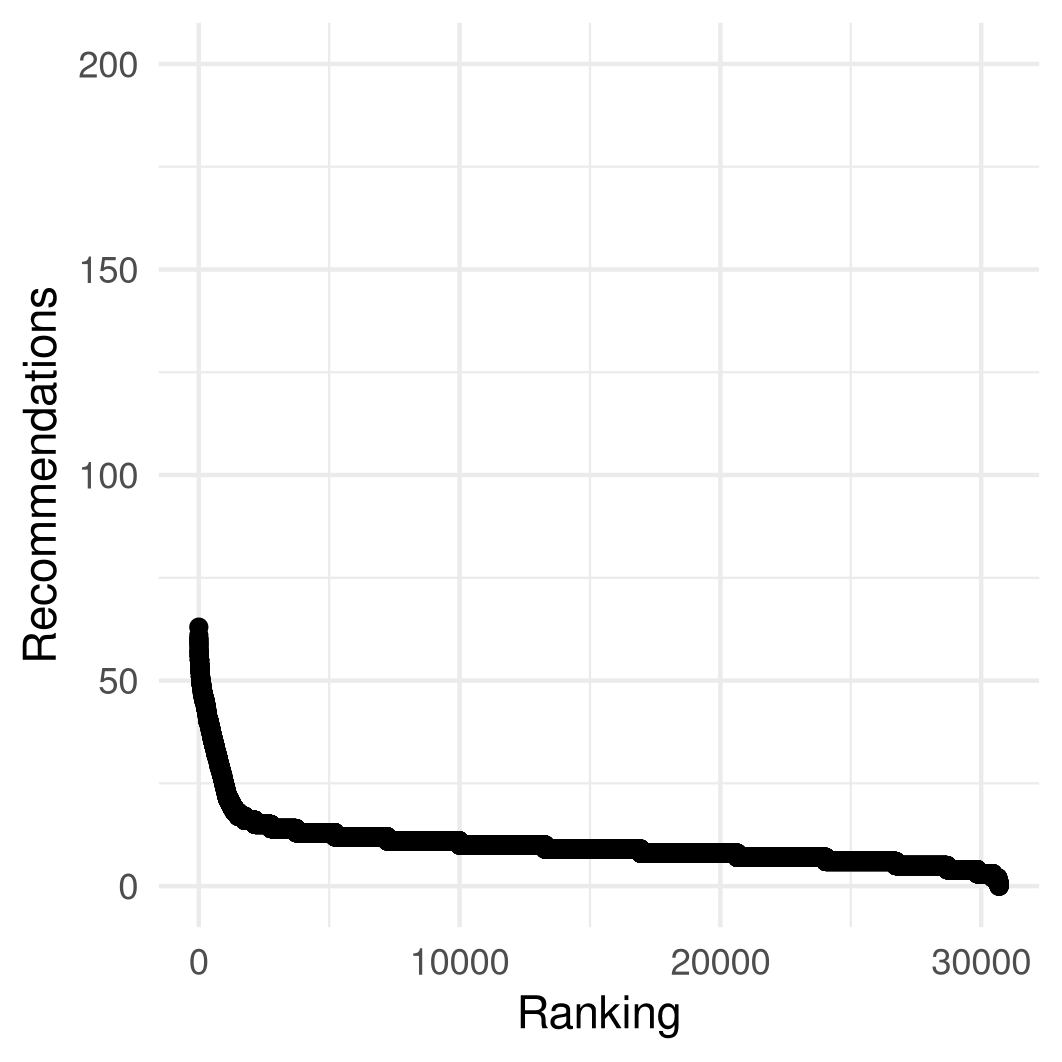
\includegraphics[width=\textwidth]{5b_p10}
    \caption{$P(w_{i}) = 10 \times \overline{P(w)}$.\label{fig:fig5b}}
  \end{subfigure}
  \begin{subfigure}{0.3\textwidth}
    \centering
    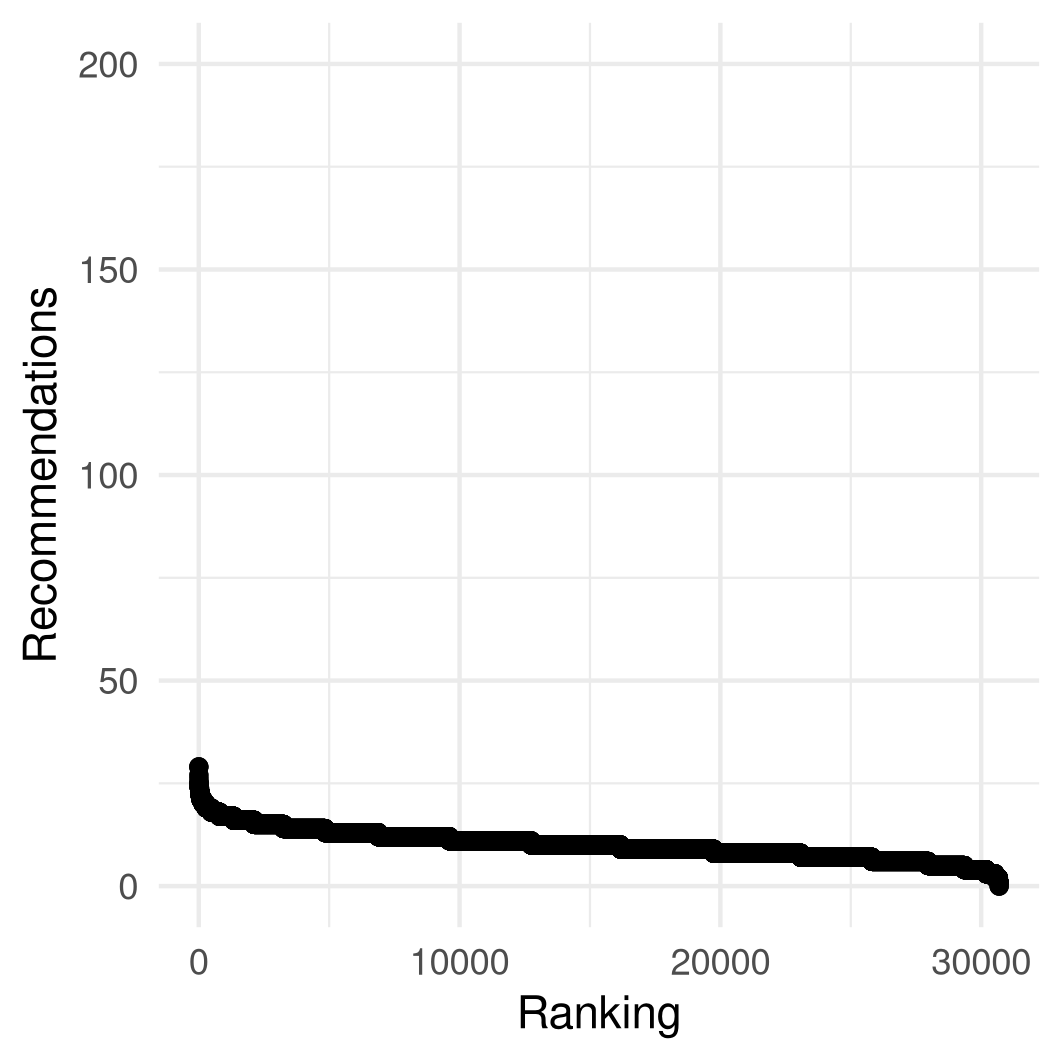
\includegraphics[width=\textwidth]{5c_p100}
    \caption{$P(w_{i}) = 100 \times \overline{P(w)}$.\label{fig:fig5c}}
  \end{subfigure}
  \caption{Recommendation profile of samples with
    $P(w_{i}) = C \times \overline{P(w)}$, $C = 1$ (a), $10$ (b), and $100$
    (c).\label{fig:fig5}}
\end{figure}

\subsection{Sanity Checks}
\label{subsec:sanity03}

After the previous experiments, sanity checks were needed in order to guarantee
that the previous hypothesis was generalizable. The first check should verify
whether an artificial movie created as a combination of the metadata from other
movies favored by the recommendation algorithm would also be favored, while the
second should check whether shorter vectors would change the decay already
observed despite being as sparse as their longer counterparts. We repeated these
tests thousands of times and the results presented below are typical of what we
found.

Figure~\ref{fig:fig6} showcases the two sanity checks. Figure~\ref{fig:fig6a}
was a model applied to the vanilla dataset with the addition of the movie
highlighted in red. As expected, this movie also showed up in the
top-recommended subset. Figure~\ref{fig:fig6b} comes from a model applied to
randomly generated vector representations in a similar fashion to the ones in
Figure~\ref{fig:fig5}, except each vector could only have 15,000 elements
instead of 55,681 (as with the vanilla model). The pattern observed before
persisted, meaning that the hypothesis still stood.

\begin{figure}
  \centering
  \begin{subfigure}{0.45\textwidth}
    \centering
    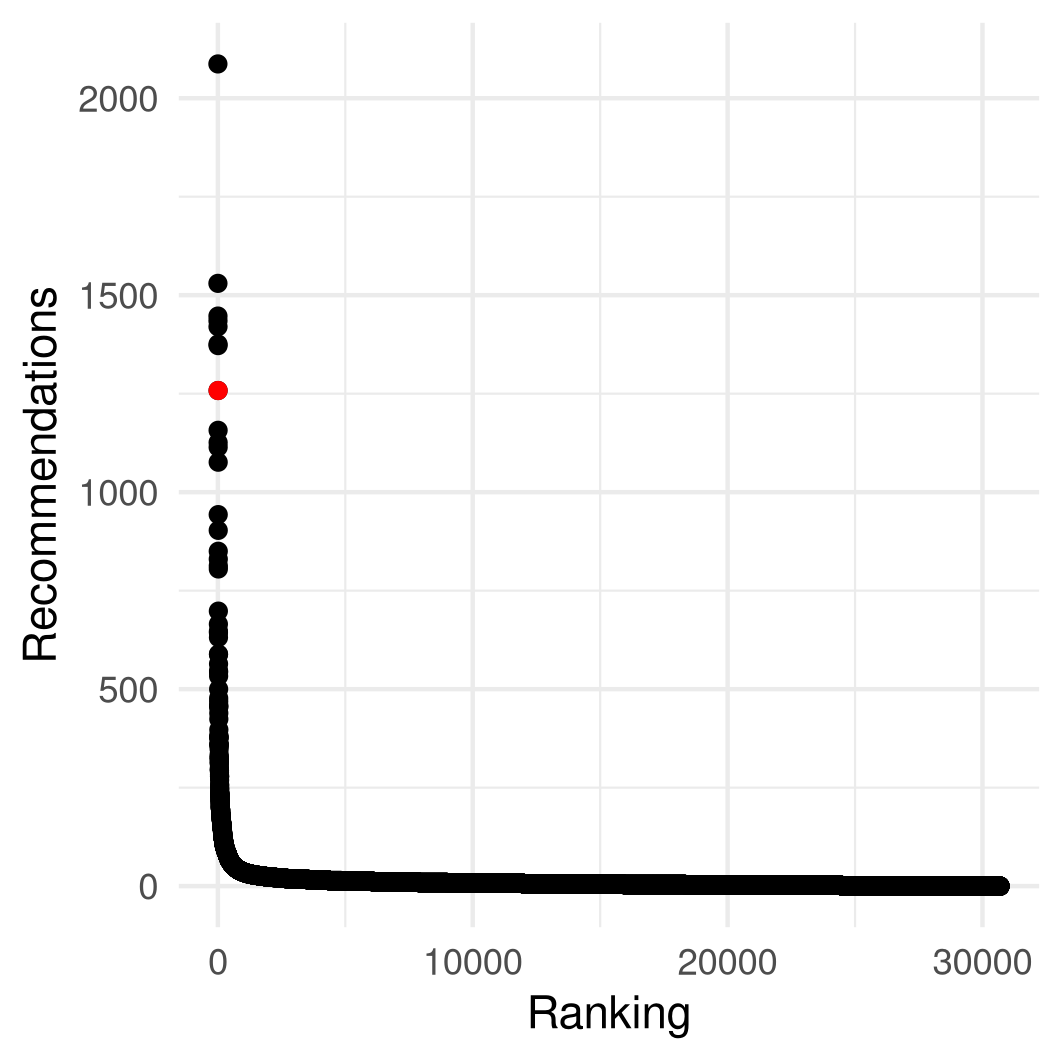
\includegraphics[width=\textwidth]{6a_artificial_movie}
    \caption{Vanilla model with artificial movie in red.\label{fig:fig6a}}
  \end{subfigure}
  \begin{subfigure}{0.45\textwidth}
    \centering
    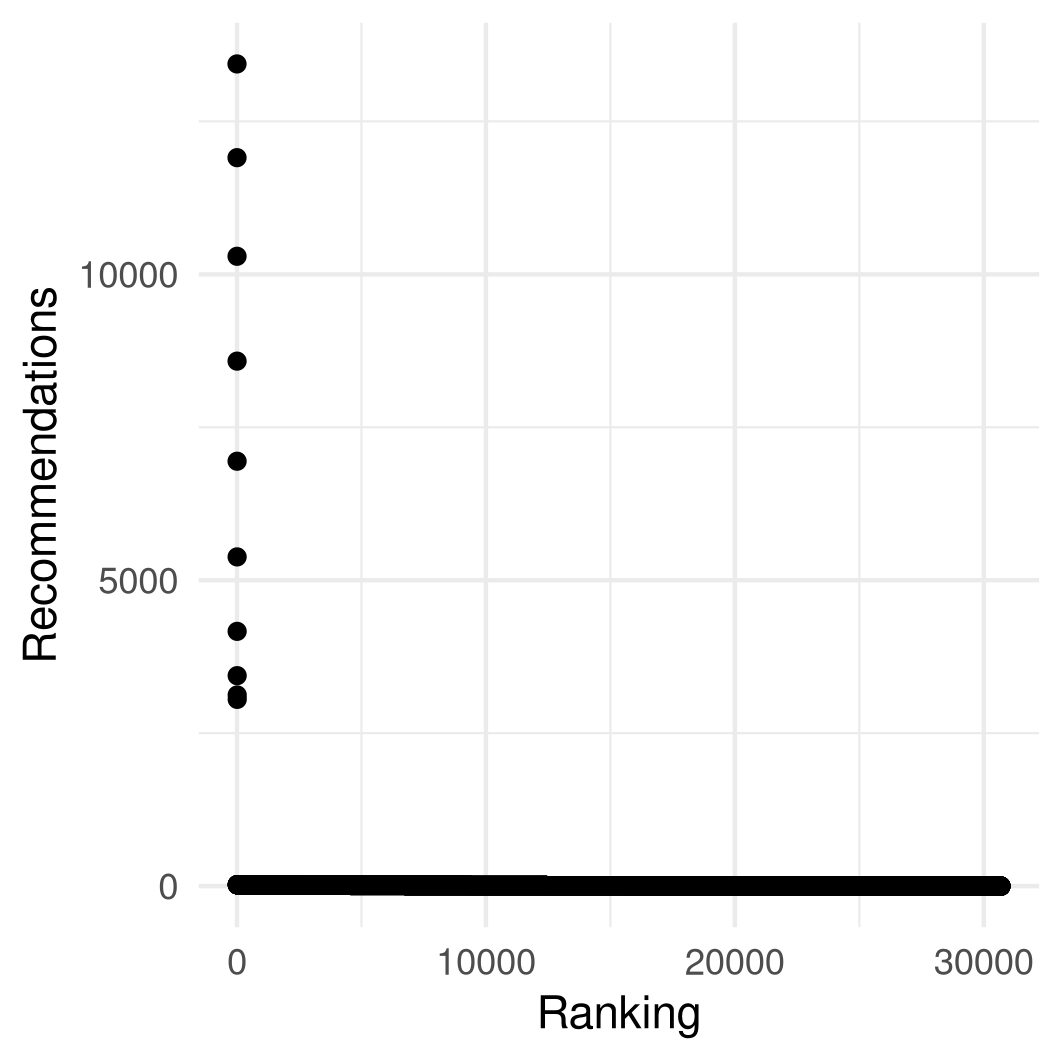
\includegraphics[width=\textwidth]{6b_long}
    \caption{Model with short vector representations.\label{fig:fig6b}}
  \end{subfigure}
  \caption{Recommendation profile for artificial movie (a) and short vector
    representations (b).\label{fig:fig6}}
\end{figure}

The last two models were considered the confirmations of the hypothesis that (at
least for this kind of recommendation systems) a subset of items was always much
more recommended than the rest as long as the data was sparse.
Figure~\ref{fig:fig7a} represents the same recommendation algorithm applied to
another dataset, the Book-Crossing dataset. Figure~\ref{fig:fig7b} contains the
results of the model applied to another set of random vector representations,
this time with the probability of each element being non-zero respecting the
marginal distributions of the vanilla dataset. Again, the exponential decay
pattern persisted, only slightly less pronounced in the Book-Crossing case.

\begin{figure}
  \centering
  \begin{subfigure}{0.45\textwidth}
    \centering
    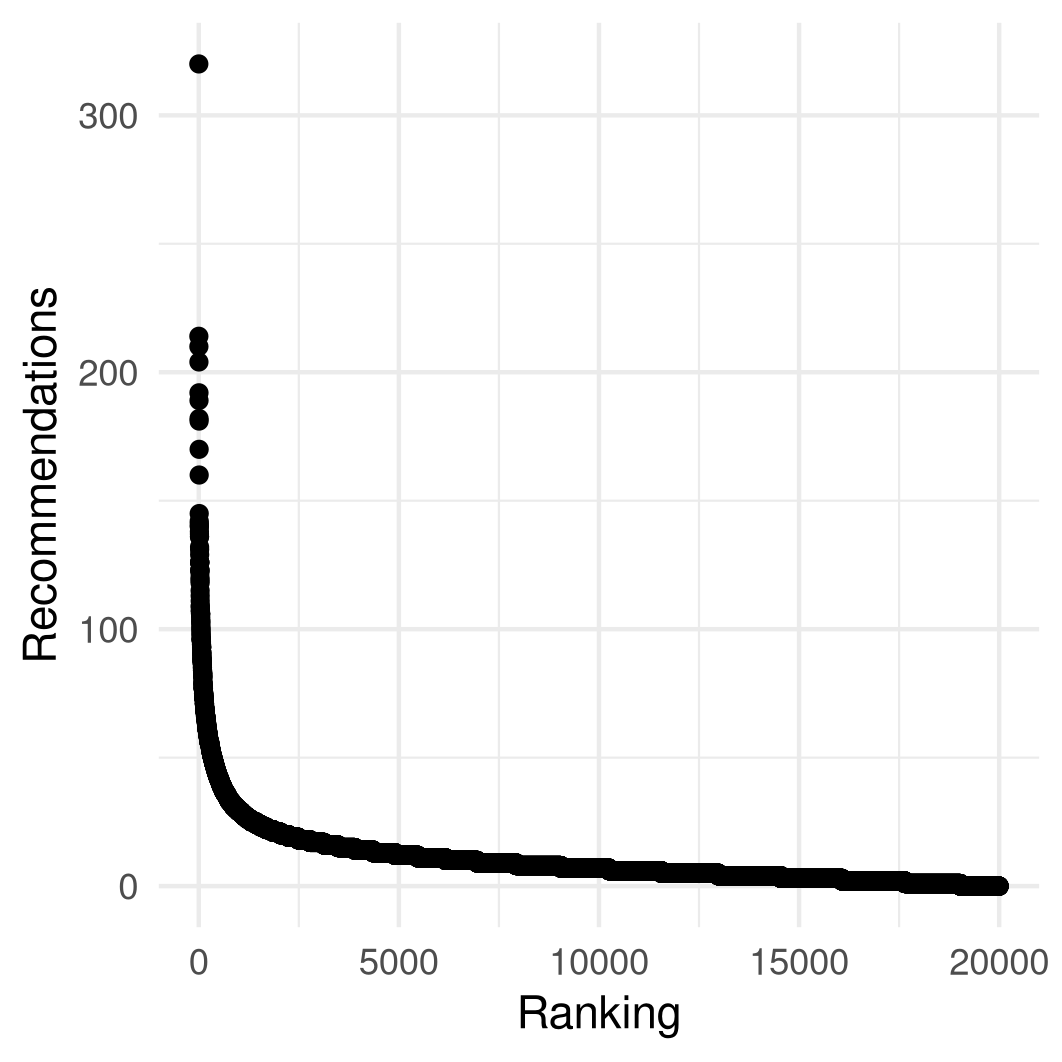
\includegraphics[width=\textwidth]{7a_books}
    \caption{Recommendation profile for book dataset.\label{fig:fig7a}}
  \end{subfigure}
  \begin{subfigure}{0.45\textwidth}
    \centering
    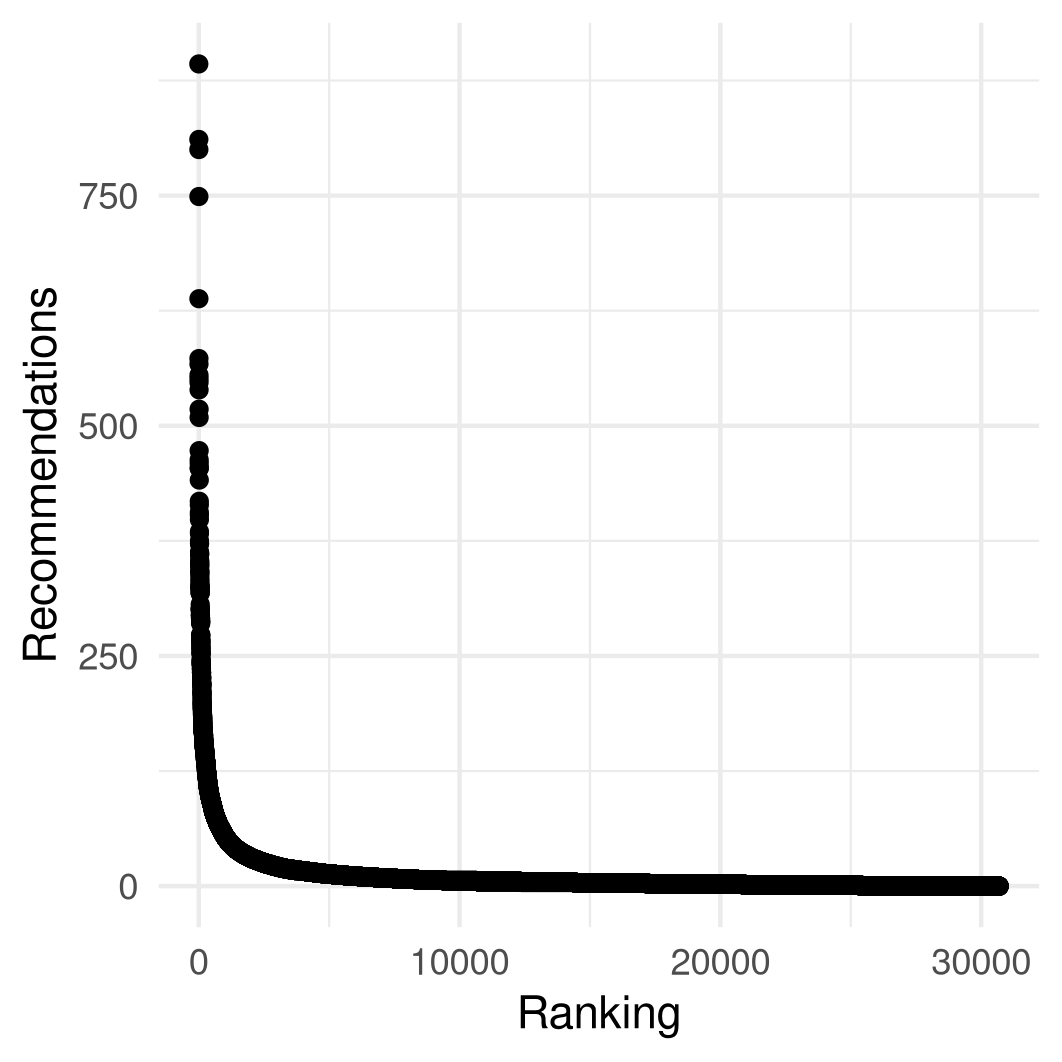
\includegraphics[width=\textwidth]{7b_mimic}
    \caption{Random simularion of vanilla.\label{fig:fig7b}}
  \end{subfigure}
  \caption{Recommendation profile for book dataset (a) and random simulation of
    vanilla (b).\label{fig:fig7}}
\end{figure}

The analysis up until now has been static, that is, the recommendation model
does not learn from the users' responses to its suggestions. There is no
interaction with users and no opportunity to evolve over time. The next chapter
addresses this point by using Google's newly released TensorFlow Recommenders
library \citep{noauthor_tensorflow_nodate} to gather data about what happens to
a system's recommendations as users follow its suggestions. Employing a deep
learning model that is able to improve over time is a significant departure from
the content-based models presented here and, if a similar recommendation profile
can also be detected for multi-criteria recommender systems on dynamic
scenarios, then the hypothesis ventilated in the section above would become even
more plausible.
